\section{Introdução}
\label{sec:introducao}

\subsection*{Definição}
%{\usebackgroundtemplate{\includegraphics[width=\paperwidth]{iot.jpg}}}
\begin{frame}{}
	\begin{block}{Internet}	
		Um vasto conjunto de redes diferentes que utilizam certos protocolos comuns e fornecem determinados serviços comuns. É um sistema pouco usual no sentido de não ter sido planejado nem ser controlado por ninguém \cite{tanenbaum2011computer}.		
	\end{block}
	
	\begin{figure}[H]
		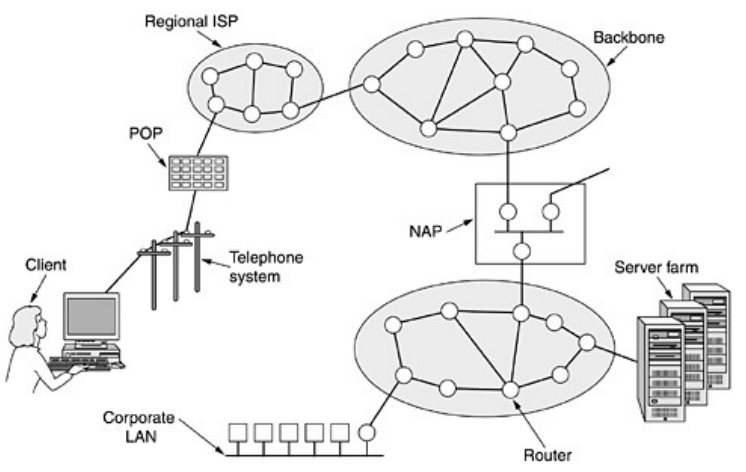
\includegraphics[width=.6\textwidth]{internet.png}\footnotemark
	\end{figure}
	
	\footnotetext{\cite{tanenbaum2011computer}}
\end{frame}

\begin{frame}{}
	\begin{block}{Coisa}	
		Tudo o que existe ou possa existir, de natureza corpórea ou incorpórea.
	\end{block}
	
	\begin{figure}[H]
		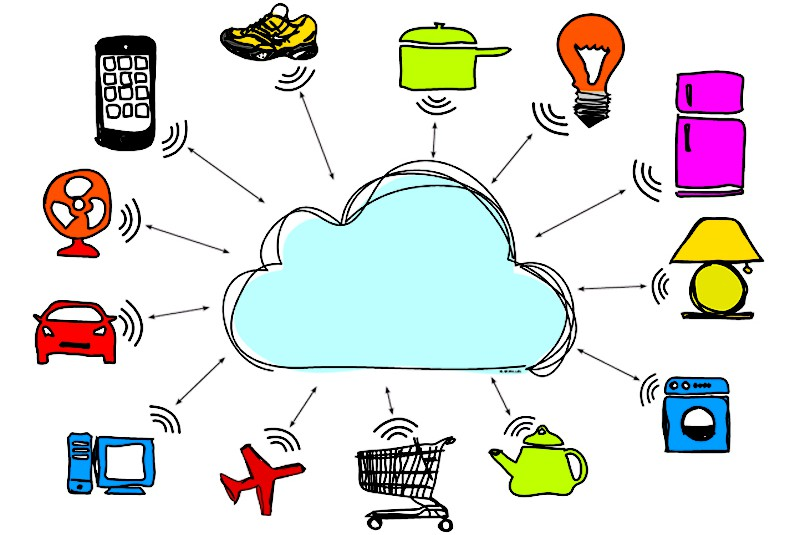
\includegraphics[width=.6\textwidth]{things.jpg}\footnotemark
	\end{figure}
	
	\footnotetext{https://www.codeproject.com/KB/Wearables/831012/}
\end{frame}

\begin{frame}{}	
	\begin{block}{Internet das Coisas}	
		Dispositivos \textbf{que falam entre si} sem intervenção humana.
	\end{block}
	
	\begin{figure}[H]
		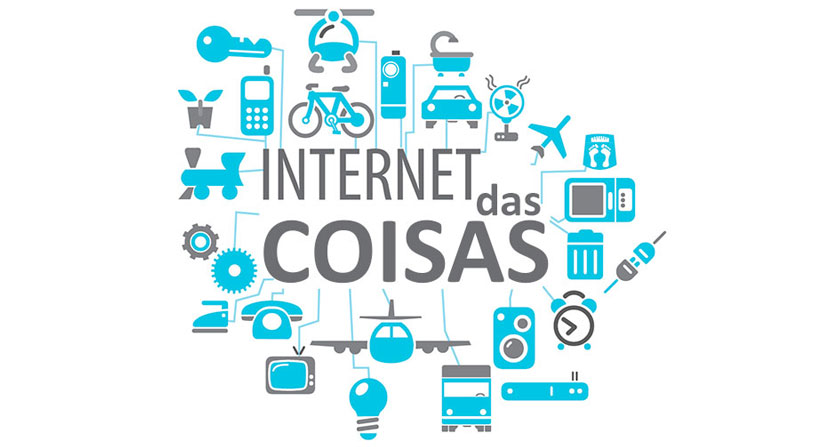
\includegraphics[width=.8\textwidth]{ioc.jpg}\footnotemark
	\end{figure}
	
	\footnotetext{http://www.blogindustrial.com.br/wp-content/uploads/2016/12/}
\end{frame}

%-------------------------------------------------
%% Objetivo:
%-------------------------------------------------
\subsection*{Objetivos}
\begin{frame}{}
	\begin{block}{Características}	
		\begin{itemize}
			\item A coisa tem que ser \textbf{única};
			\item Deve realizar processamento/\textbf{análise} de dados;
			\item Precisa \textbf{comunicar-se} com outra(s) coisa(s);
			\item Permite o \textbf{controle} da aplicação. %a qualquer hora, em qualquer lugar.
		\end{itemize}
	\end{block}
\end{frame}